\documentclass[10pt, landscape]{article}
\usepackage[scaled=0.92]{helvet}
\usepackage{calc}
\usepackage{multicol}
\usepackage[a4paper,margin=3mm,landscape]{geometry}
\usepackage{amsmath,amsthm,amsfonts,amssymb}
\usepackage{color,graphicx,overpic}
\usepackage{hyperref}
\usepackage{newtxtext} 
\usepackage{enumitem}
\usepackage[table]{xcolor}
\usepackage{mathtools}
\setlist{nosep}
% for including images
\graphicspath{ {./images/} }

\pdfinfo{
  /Title (CS3230.pdf)
  /Creator (TeX)
  /Producer (pdfTeX 1.40.0)
  /Author (Jovyn Tan)
  /Subject (CS3230)
/Keywords (CS3230, nus,cheatsheet,pdf)}

% Turn off header and footer
\pagestyle{empty}

% redefine section commands to use less space
\makeatletter
\renewcommand{\section}{\@startsection{section}{1}{0mm}%
  {-1ex plus -.5ex minus -.2ex}%
  {0.5ex plus .2ex}%x
{\normalfont\large\bfseries}}
\renewcommand{\subsection}{\@startsection{subsection}{2}{0mm}%
  {-1explus -.5ex minus -.2ex}%
  {0.5ex plus .2ex}%
{\normalfont\normalsize\bfseries}}
\renewcommand{\subsubsection}{\@startsection{subsubsection}{3}{0mm}%
  {-1ex plus -.5ex minus -.2ex}%
  {1ex plus .2ex}%
{\normalfont\small\bfseries}}%
\makeatother

\renewcommand{\familydefault}{\sfdefault}
\renewcommand\rmdefault{\sfdefault}
%  makes nested numbering (e.g. 1.1.1, 1.1.2, etc)
\renewcommand{\labelenumii}{\theenumii}
\renewcommand{\theenumii}{\theenumi.\arabic{enumii}.}
\renewcommand\labelitemii{•}
\renewcommand\labelitemiii{•}

\definecolor{mathblue}{cmyk}{1,.72,0,.38}
\everymath\expandafter{\the\everymath \color{mathblue}}

% Don't print section numbers
\setcounter{secnumdepth}{0}

\setlength{\parindent}{0pt}
\setlength{\parskip}{0pt plus 0.5ex}
%% adjust spacing for all itemize/enumerate
\setlength{\leftmargini}{0.5cm}
\setlength{\leftmarginii}{0.5cm}
\setlist[itemize,1]{leftmargin=2mm,labelindent=1mm,labelsep=1mm}
\setlist[itemize,2]{leftmargin=3mm,labelindent=1mm,labelsep=1mm}
\setlist[itemize,3]{leftmargin=3mm,labelindent=1mm,labelsep=1mm}

% adding my commands
% tightcenter
\newenvironment{tightcenter}{%
  \setlength\topsep{0pt}
  \setlength\parskip{0pt}
  \begin{center}
    }{%
  \end{center}
}

% boxed
\newenvironment{tightbox}{%
  \setlength\topsep{0pt}
  \setlength\parskip{0pt}
  \begin{center}
    \begin{tabular}{|@{\hspace{\dimexpr\fboxsep+0.5\arrayrulewidth}}c@{\hspace{\dimexpr\fboxsep+0.5\arrayrulewidth}}|}
      \hline
    }
    {%
    \\ \hline
    \end{tabular}
  \end{center}
}

% fixed width box
\newenvironment{fixedbox}[1][0.7]{
  \setlength\topsep{0pt}
  \setlength\parskip{0pt}
  \begin{center}
    \begin{tabular}{|>{\centering\arraybackslash}m{#1\linewidth}|}
    \hline
  }{
  \\ \hline
  \end{tabular}
  \end{center}
}

% definition of a new term
\usepackage{soul}
\definecolor{paleyellow}{RGB}{251,243,218}
\newcommand{\definition}[2][]{\sethlcolor{paleyellow}\hl{\textbf{#2}} #1  $\rightarrow$}

% important note (attention)
\newcommand{\attention}{{\color{red}\textbf{! }}}


\newcommand{\Mod}[1]{\ (\mathrm{mod}\ #1)}

% -----------------------------------------------------------------------

\begin{document}
\raggedright
\footnotesize
\begin{multicols*}{4}
  % multicol parameters
  \setlength{\columnseprule}{0.25pt}

  \begin{center}
    \fbox{%
      \parbox{0.8\linewidth}{\centering \textcolor{black}{
          {\Large\textbf{CS3230}}
        \\ \normalsize{AY21/22 SEM 2}}
        \\ {\footnotesize \textcolor{gray}{github/jovyntls}}
      }%
    }
  \end{center}

  \section{01. COMPUTATIONAL MODELS}
  \begin{itemize}
    \item \definition{algorithm} a well-defined procedure for finding the correct solution to the input
    \item \textbf{correctness}
      \begin{itemize}
        \item \definition{worst-case correctness} correct on \textit{every valid input}
        \item other types of correctness: correct on random input/with high probability/approximately correct
      \end{itemize}
    \item \textbf{efficiency} / \definition{running time} measures the number of steps executed by an algorithm as a function of the \textit{input size} (depends on computational model used)
      \begin{itemize}
        \item number input: typically the length of binary representation
        \item \definition[running time]{worst-case} \textit{max} number of steps executed when run on an input of size $n$ 
      \end{itemize}
  \end{itemize}

  \subsection{Comparison Model}
  \begin{itemize}
    \item algorithm can \textbf{compare} any two elements in one time unit ($x>y$, $x<y$, $x=y$)
    \item running time = number of comparisons made
    \item array can be manipulated at no cost
  \end{itemize}

  \subsubsection{Maximum Problem}
  \begin{itemize}
    \item \textit{problem}: find the largest element in an array $A$ of $n$ distinct elements
    \item \textit{proof that $n-1$ comparisons are needed}: 
      \begin{itemize}
        \item fix an algorithm $M$ that solves the Maximum problem on all inputs using $< n-1$ comparisons. construct graph $G$ where nodes $i$ and $j$ are adjacent iff $M$ compares $i$ and $j$.
          \\* 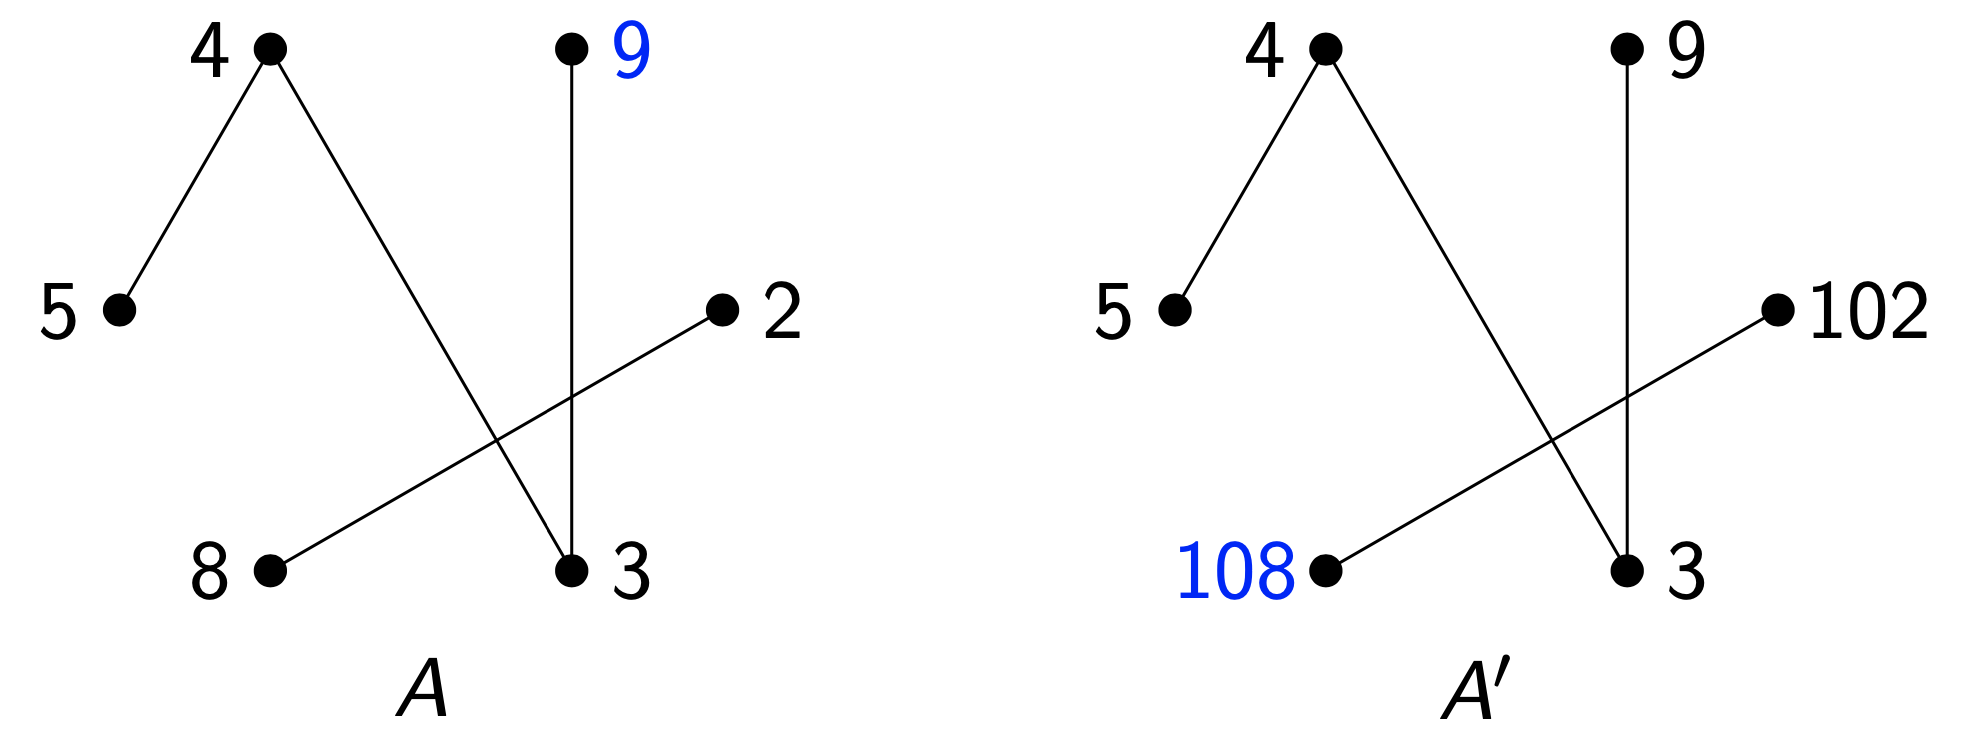
\includegraphics[width=0.7\linewidth]{maximum-problem-graph.png} 
        \item $M$ cannot differentiate $A$ and $A'$.
      \end{itemize}
    \item \definition{adversary argument} inputs are decided such that they have different solutions
  \end{itemize}

  \subsubsection{Second Largest Problem}
  \begin{itemize}
    \item \textit{problem}: find the second largest element in $<2n-3$ comparisons (2x Maximum $\Rightarrow$ $\scriptstyle (n-1) + ((n-1)-1) = 2n-3$ )
    \item \textit{solution}: \textbf{knockout tournament} $\Rightarrow n + \lceil \lg n \rceil - 2$
      \\* 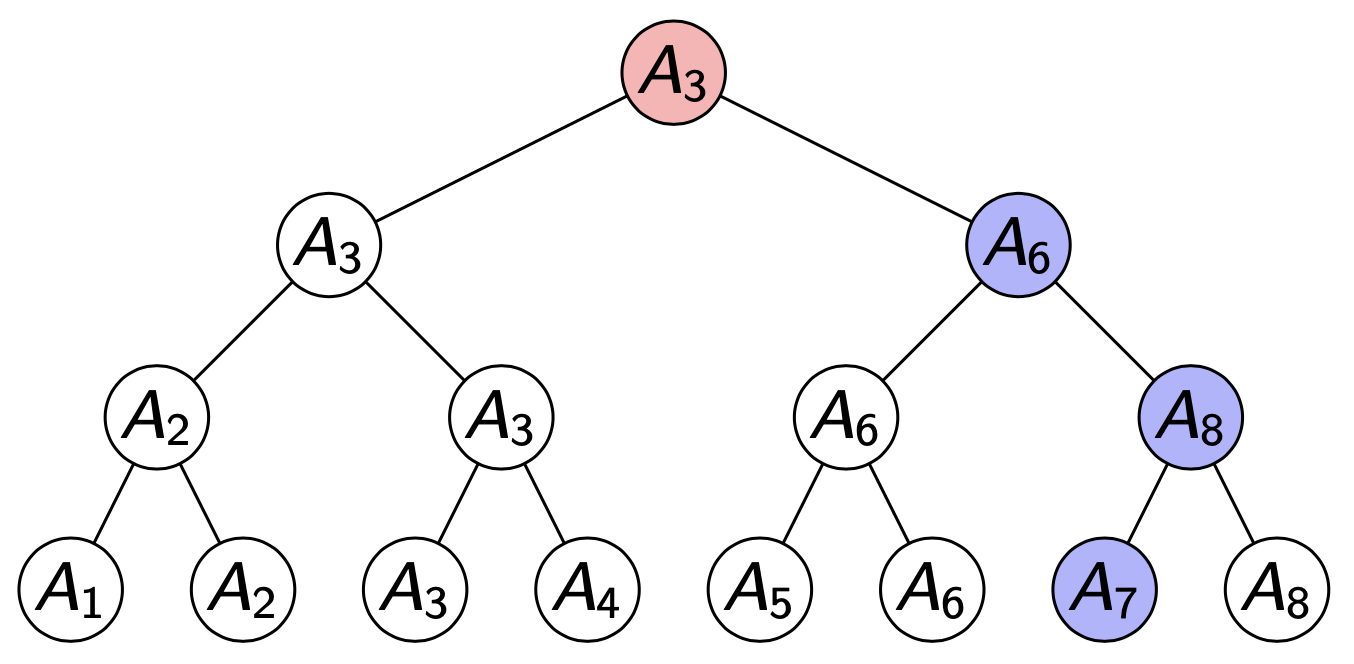
\includegraphics[width=0.6\linewidth]{second-largest-solution.png} 
      \begin{enumerate}
        \item bracket system: $n-1$ matches 
          \begin{itemize}
            \item every non-winner has lost exactly once
          \end{itemize}
        \item then compare the elements that have lost to the largest
          \begin{itemize}
            \item the second-largest element must have lost to the winner
            \item compares $\lceil \lg n \rceil$ elements that have lost to the winner using $\lceil \lg n \rceil -1$ comparisons 
          \end{itemize}
      \end{enumerate}
  \end{itemize}

  \subsubsection{Sorting}
  \begin{itemize}
    \item there is a sorting algorithm that requires $\leq n \lg n - n + 1$ comparisons.
    \item \textit{proof:} every sorting algorithm must make $\geq \lg (n!)$ comparisons.
      \begin{enumerate}
        \item let set $\mathcal{U}$ be the set of all permutations of the set $\{1, \dots, n\}$ that the adversary could choose as array $A$. $\vert \mathcal{U} \vert = n!$ 
        \item for each query "is $A_i > A_j$?", 
          \\* if $\mathcal{U}_{yes} = \{A \in \mathcal{U} : A_i > A_j\}$ is of size $\geq \vert\mathcal{U}\vert /2$, set $\mathcal{U} := \mathcal{U}_{yes}$. else: $\mathcal{U} := \mathcal{U} \backslash \mathcal{U}_{yes}$
        \item the size of $\mathcal{U}$ decreases by at most half with each comparison
        \item for $> \lg (n!)$ comparisons, $\mathcal{U}$ will still contain at least 2 permutations
      \end{enumerate}
  \end{itemize}

  \begin{tightcenter}
    $n! \geq (\frac{n}{e})^n$ 
    \\* $\Rightarrow \lg (n!) \geq n \lg (\frac{n}{e}) = n \lg n - n \lg e$
    \\* $\approx n \lg n - 1.44n$
    \\* $\Rightarrow$ roughly $n \lg n$ comparisons are \textbf{required} and \textbf{sufficient} for sorting $n$ numbers
  \end{tightcenter}

  \subsection{String Model}
  \begin{itemize}
    \item input: string of $n$ bits
    \item each query: find out \textbf{one bit} of the string
    \item $n$ queries are \textbf{necessary} and \textbf{sufficient} to check if the input string is all 0s.
  \end{itemize}

  \subsection{Graph Model}
  \begin{itemize}
    \item input: (symmetric) adjacency matrix of an $n$-node undirected graph
    \item each query: find out if an edge is present between two chosen nodes
    \item \textit{proof}: $\binom{n}{2}$ queries are necessary to decide whether the graph is connected or not
      \begin{enumerate}
        \item suppose $M$ is an algorithm making $\leq \binom{n}{2}$ queries.
        \item whenever $M$ makes a query, the algorithm tries not adding this edge, but adding all remaining unqueried edges. 
          \begin{enumerate}
            \item if the resulting graph is connected, $M$ replies $0$ (i.e. edge does not exist)
            \item else: replies $1$ (edge exists)
          \end{enumerate}
        \item after $< \binom{n}{2}$ queries, at least one entry of the adjacency matrix is unqueried.
      \end{enumerate}
  \end{itemize}


  \section{02. ASYMPTOTIC ANALYSIS}

  \begin{itemize}
    \item \definition{algorithm} a \textit{finite} sequence of well-defined instructions to solve a given computational problem
    \item \definition{runtime} measured in number of instructions taken in \textbf{word-RAM} model
      \begin{itemize}
        \item operators, comparisons, if, return, etc
      \end{itemize}
  \end{itemize}

  \subsection{Asymptotic Notations}

  \begin{tightcenter}
    \textbf{upper bound ($\leq$)}: $f(n) = O(g(n))$ 
    \\* if $\exists c>0, n_0>0$ such that $\forall n \geq n_0$, $\quad 0 \leq f(n) \leq cg(n)$ 
  \end{tightcenter}

  \begin{tightcenter}
    \textbf{lower bound ($\geq$)}: $f(n) = \Omega(g(n))$ 
    \\* if $\exists c>0, n_0>0$ such that $\forall n \geq n_0$, $\quad 0 \leq cg(n) \leq f(n)$ 
  \end{tightcenter}

  \begin{tightcenter}
    \textbf{tight bound}: $f(n) = \Theta(g(n))$ 
    \\* if $\exists c_1>0, c_2>0, n_0>0$ such that $\forall n \geq n_0, \quad 0 \leq c_1 g(n) \leq f(n) \leq c_2 g(n)$ 
  \end{tightcenter}

  \begin{tightcenter}
    \textbf{$o$ notation ($<$)}: $f(n) = o(g(n))$ 
    \\* if $\forall c>0, \exists n_0>0$ such that $\forall n \geq n_0$, $\quad 0 \leq f(n) < cg(n)$ 
  \end{tightcenter}

  \begin{tightcenter}
    \textbf{$\omega$-notation ($>$)}: $f(n) = \omega(g(n))$ 
    \\* if $\forall c>0, \exists n_0>0$ such that $\forall n \geq n_0$, $\quad 0 \leq cg(n) < f(n)$ 
  \end{tightcenter}

  \subsubsection{Set definitions}

  \begin{itemize}
    \item \textit{upper}: $O(g(n)) = $
      \\* $ \{f(n): \exists c>0, n_0>0 \mid \forall n \geq n_0, \, 0 \leq f(n) \leq cg(n)\}$
    \item \textit{lower}: $\Omega(g(n)) = $
      \\* $ \{f(n): \exists c>0, n_0>0 \mid \forall n \geq n_0, \, 0 \leq cg(n) \leq f(n)\}$
  \end{itemize}

  \begin{niceproof}
    that $2n^2 = O(n^3)$ 
    \\* let $f(n) = 2n^2$. then $f(n) = 2n^2 \leq n^3$ when $n \geq 2$. 
    \\* set  $c=1$ and $n_0 = 2$.
    \\* we have $f(n) = 2n^2 \leq c \cdot n^3$ for $n \geq n_0$. \qed
  \end{niceproof}

  \subsection{Limits}

  Assume $f(n), g(n) > 0$.
  \begin{center}
    $\lim\limits_{n \to \infty} \frac{f(n)}{g(n)} = 0 \Rightarrow f(n) = o(g(n))$
    \\* $\lim\limits_{n \to \infty} \frac{f(n)}{g(n)} < \infty \Rightarrow f(n) = O(g(n))$
    \\* $0 < \lim\limits_{n \to \infty} \frac{f(n)}{g(n)} < \infty \Rightarrow f(n) = \Theta(g(n))$
    \\* $\lim\limits_{n \to \infty} \frac{f(n)}{g(n)} > 0 \Rightarrow f(n) = \Omega(g(n))$
    \\* $\lim\limits_{n \to \infty} \frac{f(n)}{g(n)} = \infty \Rightarrow f(n) = \omega(g(n))$
  \end{center}

  \begin{niceproof}
    using delta epsilon definition
  \end{niceproof}

  \subsection{Properties of Big O}

  \begin{fixedbox}
    $\Theta(g(n)) = O(g(n)) \cap \Omega(g(n))$
  \end{fixedbox}

  \begin{itemize}
    \item $\textbf{transitivity}$ - applies for $O, \Theta, \Omega, o, \omega$
      $f(n) = O(g(n)) \land g(n) = O(h(n)) \Rightarrow f(n) = O(h(n))$ 
    \item \textbf{reflexivity} - for $O, \Omega, \Theta, \quad f(n) = O(f(n))$ 
    \item \textbf{symmetry} - $f(n) = \Theta(g(n)) \iff g(n) = \Theta(f(n))$
    \item \textbf{complementarity} - 
      \begin{itemize}
        \item $f(n) = O(g(n)) \iff g(n) = \Omega(f(n))$
        \item $f(n) = o(g(n)) \iff g(n) = \omega(f(n))$
      \end{itemize}
  \end{itemize}

  insertion sort: $O(n^2)$ with worst case $\Theta(n^2)$

  \begin{fixedbox}[0.8]
    $\log\log n < \log n < (\log n)^k < n^k < k^n$
  \end{fixedbox}

  \section{03. ITERATION, RECURSION, DIVIDE-AND-CONQUER}

  \subsection{Iterative Algorithms}

  \textbf{loop invariant} implies correctness if 
  \begin{itemize}
    \item \textit{initialisation} - true before the first iteration
    \item \textit{maintenance} - if true before an iteration, remains true at the beginning of the next iteration
    \item \textit{termination} - true at the end
  \end{itemize}

  \subsection{Divide-and-Conquer}

  \subsubsection{powering a number}

  \begin{itemize}
    \item problem: compute $f(n, m) = a^n\Mod{m}$ for all integer $n, m$
    \item observation: $f(x+y, m) = f(x, m) * f(y, m) \Mod{m}$
    \item \textbf{naive solution}: recursively compute and combine $f(n-1, m) * f(1, m) \Mod m$ 
      \begin{itemize}
        \item $T(n) = T(n-1) + T(1) + \Theta(1) \Rightarrow T(n) = \Theta (n)$
      \end{itemize}
    \item \textbf{better solution}: divide and conquer
      \begin{itemize}
        \item divide: trivial
        \item conquer: recursively compute $f(\lfloor n / 2 \rfloor, m)$ 
        \item combine: 
          \begin{itemize}
            \item $f(n, m) = f(\lfloor n / 2 \rfloor, m)^2 \Mod m$ if n is even
            \item $f(n, m) = f(1, m) * f(\lfloor n / 2 \rfloor, m)^2 \Mod m$ if odd
          \end{itemize}
        \item $T(n) = T(n/2) + \Theta(1) \Rightarrow \Theta(\log n)$
      \end{itemize}
  \end{itemize}

  \section{Solving Recurrences}
  for $a$ sub-problems of size $\frac{n}{b}$ where $f(n)$ is the time to divide and combine,
  \begin{math}
    T(n) = aT(\frac{n}{b}) + f(n)
  \end{math}

  \subsection{Recursion tree}
  total = height $\times$ number of leaves
  \begin{tightcenter}
    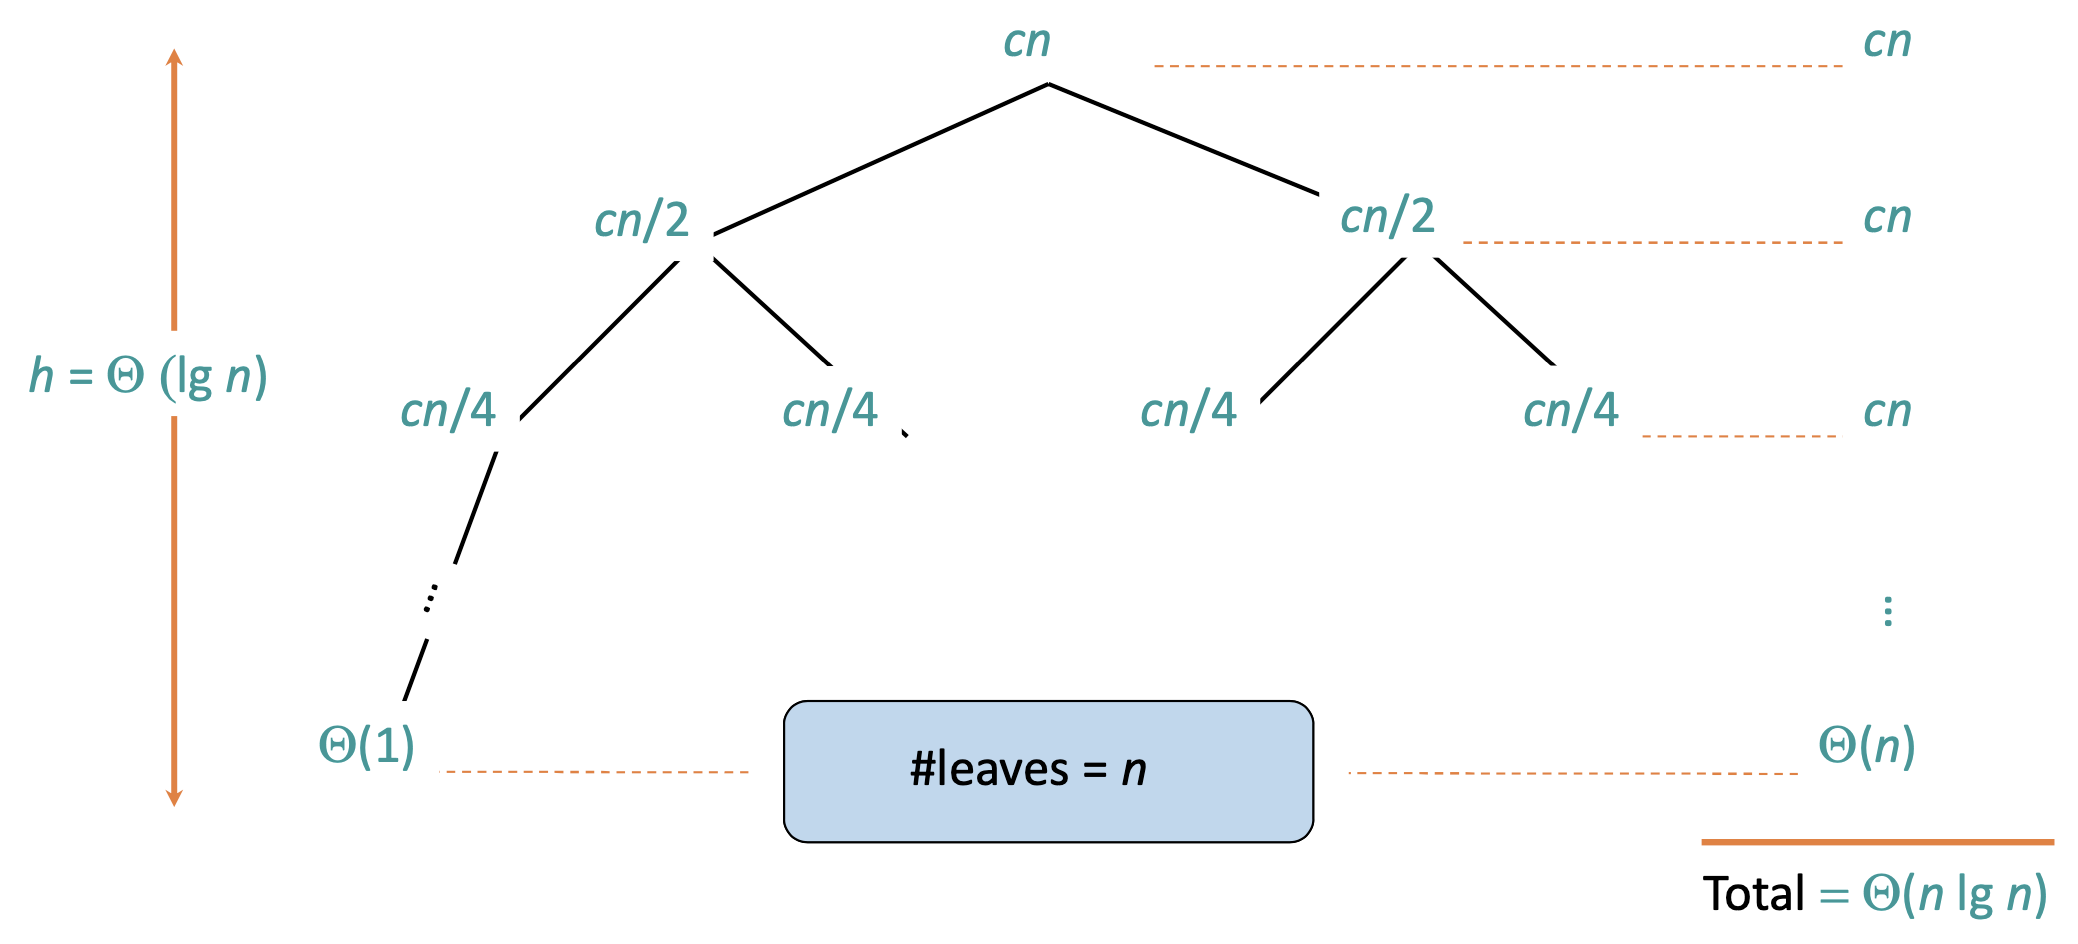
\includegraphics[width=0.9\linewidth]{cs3230-recursion-tree-example-1.png} 
    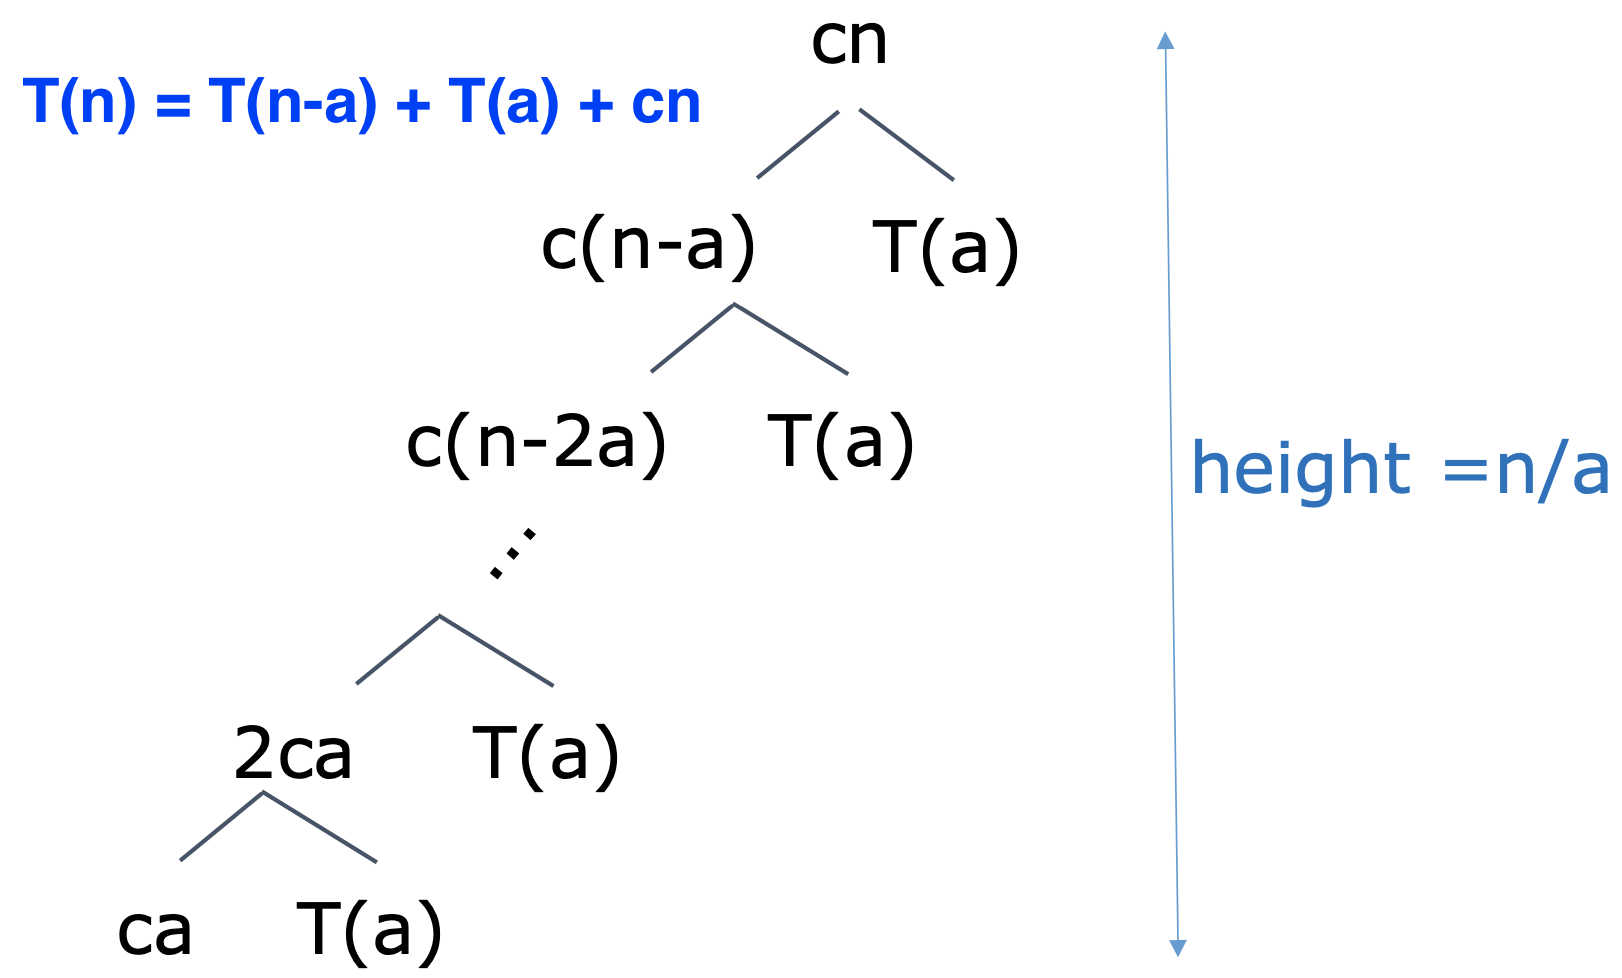
\includegraphics[width=0.6\linewidth]{cs3230-recursion-tree-example-2.png} 
  \end{tightcenter}

  \subsection{Master method}
  $T(n) = aT(\frac{n}{b}) + f(n)$
  \\ $a \geq 0, b > 1, f$ is asymptotically positive

  \begin{math}
    T(n) = \begin{cases}
      \Theta(n^{\log_ba}) & \text{ if } f(n) < n^{\log_ba} \text{ polynomially}
      \\ \Theta(n^{\log_ba} \log n) & \text{ if } f(n) = n^{\log_ba} 
      \\ \Theta(f(n)) & \text{ if } f(n) > n^{\log_ba} \text{ polynomially}
    \end{cases}
  \end{math}

  \textbf{harmonic series}: $\sum\limits^\infty_{k=1} \frac{1}{k} \approx \ln k = \Theta (\lg n)$

  \subsection{Substitution method}
  \begin{enumerate}
    \item guess that $T(n) = O(f(n))$. 
      \\* i.e. $\exists c$ such that $T(n) \leq c \cdot f(n)$, for $n \geq n_0$.
    \item verify by induction:
      \begin{enumerate}
        \item set $c = \max\{2, q\}$ and $n_0 = 1$
        \item base case ($n = n_0 = 1$)
        \item recursive case ($n > 1$):
          \begin{itemize}
            \item by strong induction, assume $T(k) = c \cdot f(k)$ for $n > k > 1$
            \item T(n) = <recurrence> ... $\leq c \cdot f(n)$
          \end{itemize}
        \item hence $T(n) \leq c \cdot f(n)$ for $n \geq 1$.
      \end{enumerate}
  \end{enumerate}
  \attention may not be a tight bound!

  \subsubsection{example}

  $T(n) = 4T(n/2) + n^2/\lg n \Rightarrow \Theta(n^2\lg \lg n)$

  \begin{niceproof}
    $T(n) = 4T(n/2) + \frac{n^2}{\lg n}$ \\
    $= 4( 4T(n/4) + \frac{(n/2)^2}{\lg n - lg 2} ) + \frac{n^2}{\lg n}$ \\ 
    $= 16 T(n/4) + \frac{n^2}{\lg n - \lg 2} + \frac{n^2}{\lg n}$ \\
    $= \sum\limits^{\lg n}_{k=1} \frac{n^2}{\lg n - k}$ \\
    $= n^2 \lg \lg n$ by approx. of harmonic series ($\sum\frac{1}{k}$)
  \end{niceproof}

  \section{04. AVERAGE-CASE ANALYSIS \& RANDOMISED ALGORITHMS}

  \subsection{Quicksort Analysis}

  \begin{itemize}
    \item divide \& conquer, linear-time $\Theta(n)$ partitioning subroutine
    \item assume we select the first array element as pivot 
    \item if the pivot produces subarrays of size $j$ and $(n-j-1)$, then $T(n) = T(j) + T(n-j-1) + \Theta(n)$
  \end{itemize}

  \textbf{time analysis}
  \begin{itemize}
    \item \textbf{worst-case}: $T(n) = T(0) + T(n-1) + \Theta(n) \Rightarrow \Theta(n^2)$ 
    \item \definition[$A(n)$]{average case} expected running time when the input is chosen uniformly at random from the set of all $n!$ permutations
    \item \textbf{average case}, $A(n) = \frac{1}{n!} \sum_\pi Q(\pi)$ where $Q(\pi)$ is the time complexity when the input is permutation $\pi$.
  \end{itemize}

  \begin{niceproof}
    for quicksort, $A(n) = O(n \log n)$

    let $P(i)$ be the set of all those permutations of elements $\{e_1, e_2, \dots, e_n\}$ that begins with $e_i$.

    Let $G(n, i)$ be the average running time of quicksort over $P(i)$.
    Then $G(n) = A(i-1) + A(n-i) + (n-1)$.
    $A(n) = \frac{1}{n} \sum_{i=1}^n G(n, i)$
    \\ $\quad\quad = \frac{1}{n} \sum_{i=1}^n ( A(i-1) + A(n-i) + (n-1) )$
    \\ $\quad\quad = \frac{2}{n} \sum_{i=1}^n A(i-1)+n-1$
    \\ $\quad\quad = O(n\log n)$ by taking it as area under integration
  \end{niceproof}

  \subsubsection{quicksort vs mergesort}

  \begin{center}
    \begin{tabular}{|c|c|c|c|}
      \hline
      & average & best & worst \\\hline
      quicksort & $1.39n\lg n$ &  $n \lg n$ & $n(n-1)$ \\\hline
      mergesort & $n\lg n$ &  $n \lg n$ & $n \lg n$ \\\hline
    \end{tabular}
  \end{center}

  \begin{itemize}
    \item disadvantages of mergesort:
      \begin{itemize}
        \item overhead of temporary storage
        \item cache misses
      \end{itemize}
    \item advantages of quicksort
      \begin{itemize}
        \item in place
        \item reliable (as $n \uparrow$, chances of deviation from avg case $\downarrow$)
      \end{itemize}
    \item issues with quicksort
      \begin{itemize}
        \item \definition{distribution-sensitive} time taken depends on the initial (input) permutation
      \end{itemize}
  \end{itemize}

  \subsection{Randomised Algorithms}

  \begin{itemize}
    \item \definition{randomised algorithms} output and running time are \textbf{functions} of the \textbf{input} and \textbf{random bits chosen}
      \begin{itemize}
        \item vs non-randomised: output \& running time are functions of the \textit{input only}
      \end{itemize}
    \item \textbf{randomised quicksort}: choose pivot at random 
      \begin{itemize}
        \item probability that the runtime of \textit{randomised} quicksort exceeds average by $x\% = n^{-\frac{x}{100}\ln\ln n}$ 
        \item P(time takes at least double of the average) = $10^{-15}$
        \item distribution insensitive
      \end{itemize}
  \end{itemize}

  \subsubsection{Randomised Quicksort Analysis}

  $T(n) = n-1 + T(q-1) + T(n-q)$

  Let $A(n) = \mathbb{E}[T(n)]$ where the expectation is over the randomness in expectation.

  Taking expectations and applying linearity of expectation:
  $A(n) = n-1 + \frac{1}{n} \sum^n_{q=1} (A(q-1) + A(n-q)) $ 
  $\;\quad\quad = n-1 + \frac{2}{n} \sum\limits^{n-1}_{q=1} A(q) $ 

  $A(n) = n \log n \quad \Rightarrow$ same as average case quicksort

  \subsubsection{Randomised Quickselect}

  \begin{itemize}
    \item $O(n)$ to find the $k^{th}$ smallest element
    \item randomisation: unlikely to keep getting a bad split
  \end{itemize}

  \subsubsection{Types of Randomised Algorithms}

  \begin{itemize}
    \item randomised \textbf{Las Vegas} algorithms
      \begin{itemize}
        \item output is always correct
        \item runtime is a \textit{random variable} 
        \item e.g. randomised quicksort
      \end{itemize}
    \item randomised \textbf{Monte Carlo} algorithms
      \begin{itemize}
        \item output may be incorrect with some small probability
        \item runtime is \textit{deterministic}
      \end{itemize}
  \end{itemize}

  \textbf{examples}
  \begin{itemize}
    \item \textit{smallest enclosing circle:} given $n$ points in a plane, compute the smallest radius circle that encloses all $n$ points
      \begin{itemize}
        \item best \textbf{deterministic} algorithm: $O(n)$, but complex
        \item las vegas: average $O(n) $, simple solution
      \end{itemize}
    \item \textit{minimum cut:} given a connected graph $G$ with $n$ vertices and $m$ edges, compute the smallest set of edges whose removal would disconnect $G$.
      \begin{itemize}
        \item best \textbf{deterministic} algorithm: $O(mn)$
        \item \textbf{monte carlo}: $O(m \log n) $, error probability $n^{-c}$ for any $c$
      \end{itemize}
    \item \textit{primality testing:} determine if an $n$ bit integer is prime
      \begin{itemize}
        \item best \textbf{deterministic} algorithm: $O(n^6)$
        \item \textbf{monte carlo}: $O(kn^2)$, error probability $2^{-k}$ for any $k$
      \end{itemize}
  \end{itemize}

  \subsection{Geometric Distribution}

  Let $X$ be the number of trials repeated until success. 

  $X$ is a random variable and follows a geometric distribution with probability $p$.

  \begin{tightcenter}
    Expected number of trials, $E[X] = \frac{1}{p} $
    \\* $ Pr[X=k] = q^{k-1}p $
  \end{tightcenter}

  \subsubsection{Linearity of Expectation}

  For any two events $ X, Y $ and a constant $ a $, 
  \begin{tightcenter}
    $ E[X+Y] = E[X] + E[Y] $
    \\ $ E[aX] = aE[X] $
  \end{tightcenter}

  \subsubsection{Coupon Collector Problem}

  \textit{$ n $ types of coupon are put into a box and randomly drawn with replacement.
  What is the expected number of draws needed to collect at least one of each type of coupon?}

  \begin{itemize}
    \item let $ T_i $ be the time to collect the $ i $-th coupon after the $ i-1 $ coupon has been collected. 
      \begin{itemize}
        \item Probability of collecting a new coupon, $ p_i = \frac{(n-(i-1))}{n}  $
        \item $ T_i $ has a \textbf{geometric distribution}
        \item $ E[T_i] = 1/p_i $
      \end{itemize}
    \item total number of draws, $ T = \sum\limits^n_{i=1} T_i $
    \item $ E[T] = E[\sum\limits^n_{i=1}T_i] = \sum\limits^n_{i=1}E[T_i] $ by linearity of expectation
      \\* $ = \sum\limits^n_{i=1} \frac{n}{n-(i-1)} = n \cdot \sum\limits^n_{i=1} \frac{1}{i} = \Theta(n \lg n) $
  \end{itemize}























\end{multicols*}

\pagebreak

\section{helpful approximations}
harmonic number, $ H_n = \sum\limits_{k=1}^n \frac{1}{k} = \Theta(\lg n) $

\end{document}
